\documentclass[conference]{IEEEtran}

\usepackage[utf8]{inputenc}
\usepackage[T1]{fontenc}
\usepackage{cite}
\usepackage{amsmath,amssymb,amsfonts}
\usepackage{algorithm}
\usepackage{algpseudocode}
\usepackage{graphicx}
\usepackage{booktabs}
\usepackage{tabularx}
\usepackage{array}
\usepackage{xcolor}
\usepackage{tikz}
\usetikzlibrary{arrows.meta,positioning,shapes.geometric,fit,backgrounds}
\usepackage{url}
\usepackage[hidelinks]{hyperref}

\newcolumntype{L}[1]{>{\raggedright\arraybackslash}p{#1}}
\newcolumntype{Y}{>{\raggedright\arraybackslash}X}

\begin{document}

\title{AirGuard AI: A Deterministic and Row-Level Provenance-Grounded Conversational Agent for Taiwan Air Quality Analysis}

\author{
\IEEEauthorblockN{Ching-Hsiang Hsu, Chun-Wei Li, and Cheng-Che Wu}
\IEEEauthorblockA{Department of Information and Computer Science (Placeholder Affiliation)\\
University Name Placeholder, Taiwan\\
Email: \{chhsu, cwli, ccwu\}@example.edu.tw}
}

\maketitle

\begin{abstract}
Air pollution remains a leading environmental threat to global public health, with the \emph{State of Global Air 2025} report attributing 7.9 million deaths worldwide (approximately one in eight deaths) to pollutant exposure and the World Health Organization (WHO) noting that 99\% of the global population breathes air exceeding guideline limits. In Taiwan, the Ministry of Environment (MOENV) tightened national air quality standards effective January 1, 2025---lowering the annual $\text{PM}_{2.5}$ threshold from 15 to $12\,\mu\text{g/m}^3$, enforcing station-by-station compliance, and advancing Air Quality Index (AQI) warnings---while afternoon photochemical ozone ($\text{O}_3$) increasingly drives Orange Alerts (AQI 101--150) across lee-side western basins. Although MOENV releases hourly historical station records (\texttt{AQX\_P\_488}), public and analytical usability is hindered by raw data inconsistencies, complex statutory sub-index rules, and the tendency of standalone large language models (LLMs) to hallucinate numeric values or emit unverified causal and clinical claims. To address these challenges, this paper proposes \textbf{AirGuard AI}, a domain-specific, provenance-grounded conversational AI agent that strictly decouples natural language orchestration from deterministic analytics. Based on a reproducible audit of 970,296 raw hourly observations (January--October 2026), the data pipeline resolves localized duplicates, recovers four uniquely mappable station identifiers, quarantines 13 conflicting station-time keys (26 variants), and establishes a single source of truth containing 606,137 unique records across 88 stations. During inference, a constrained LLM planner extracts structured query parameters and invokes deterministic Python tools, Taiwan MOENV maximum-sub-index AQI rules, a 75\% daily temporal coverage validator, and a mandatory row-level provenance guard binding every numeric claim to its \texttt{(SiteId, DataCreationDate, SourceRowID)}. Furthermore, a scope guard enforces explicit abstention on industrial causal attribution and individualized medical diagnosis. A fixed 60-question benchmark (\texttt{AirGuard-Eval-60}) comprising 45 answerable queries and 15 boundary/abstention cases is designed to evaluate LLM-only baselines, deterministic tools alone, and the proposed agent on numeric accuracy, provenance linkage, unsupported-claim suppression, and abstention precision.
\end{abstract}

\begin{IEEEkeywords}
Air quality index (AQI), conversational AI, deterministic analytics, domain-specific AI agents, evidence grounding, large language models, provenance tracking, safety-aware systems.
\end{IEEEkeywords}

\section{Introduction}
Ambient air pollution continues to impose severe global mortality and morbidity burdens. According to the Health Effects Institute (HEI) \emph{State of Global Air 2025} report~\cite{hei2025soga}, roughly 7.9 million deaths worldwide---approximately one in eight global deaths, with 86\% (6.8 million) linked to noncommunicable diseases such as heart disease, stroke, and chronic obstructive pulmonary disease---are attributable to air pollution exposure. Complementing this finding, the World Health Organization (WHO) 2025 science and policy summary (Ref.~B09461)~\cite{who2025summary} reports that 99\% of the global population resides in areas exceeding WHO Air Quality Guidelines~\cite{who2021guidelines}.

In Taiwan, East Asian monsoon circulations, central mountain range topography, and dense western industrial-urban emissions create pronounced spatiotemporal air-quality variability. Effective January 1, 2025, Taiwan's Ministry of Environment (MOENV) enacted stricter national Air Quality Standards~\cite{moenv2025standards}, reducing the annual $\text{PM}_{2.5}$ threshold from 15 to $12\,\mu\text{g/m}^3$, lowering the 24-hour $\text{PM}_{2.5}$ limit from 35 to $30\,\mu\text{g/m}^3$, enforcing station-by-station attainment rather than regional averaging, and triggering AQI advisories two to four hours earlier. Despite steady multi-year declines in national mean $\text{PM}_{2.5}$ to approximately $12.5\text{--}12.6\,\mu\text{g/m}^3$, 14 counties remain classified as Class-3 $\text{PM}_{2.5}$ non-attainment zones under the 2025 standard, while afternoon photochemical ozone ($\text{O}_3$) under weak lee-side winds has become a primary driver of Orange Alerts (AQI 101--150) across central and southern basins~\cite{moenv2025standards,moenv2025ozone}.

Although MOENV publishes hourly historical station observations via the open dataset \texttt{AQX\_P\_488} covering 88 monitoring stations~\cite{moenv_aqx_p_488,moenv_aqi_def}, general users and researchers face four structural barriers when posing natural-language analytical queries (e.g., comparing afternoon ozone surges and governing pollutants across neighboring stations):
\begin{enumerate}
    \item \textbf{Raw Open-Data Noise and Key Conflicts:} A reproducible audit of 10 monthly \texttt{AQX\_P\_488} CSV archives spanning January 1 to October 29, 2026 (16:00) reveals 970,296 raw rows containing bilingual Chinese/English duplicate headers, 364,146 duplicate rows, sentinel missing strings (\texttt{-}, \texttt{--}, \texttt{NA}), four rows missing \texttt{SiteId}, and 13 conflicting \texttt{(SiteId, DataCreationDate)} keys (26 contradictory variants across \texttt{AQI}, \texttt{PM2.5\_AVG}, and \texttt{PM10\_AVG})~\cite{moenv_aqx_p_488}. Naive ingestion or silent averaging corrupts downstream statistics.
    \item \textbf{LLM Table Faithfulness Hallucinations:} Recent benchmarks including TableBench~\cite{wu2024tablebench} and RAGTruth~\cite{niu2024ragtruth} demonstrate that standalone or unconstrained retrieval-augmented LLMs frequently misalign table rows, exhibit arithmetic drift during multi-row aggregations, and fabricate ungrounded citations.
    \item \textbf{Regulatory Semantic Complexity:} Statutory MOENV AQI calculation takes the maximum sub-index across six criteria pollutants evaluated over distinct averaging windows (e.g., hourly \texttt{O3} versus 8-hour moving-average \texttt{O3\_8hr}, and \texttt{PM2.5\_AVG})~\cite{moenv_aqi_def}, requiring strict temporal alignment and a 75\% daily completeness gate ($\ge 18/24$ valid hours).
    \item \textbf{Out-of-Bounds Attribution and Clinical Risks:} Fixed ambient stations reflect regional background concentrations rather than personal inhaled exposure~\cite{usepa_siting,who2025summary}, and spatiotemporal correlations cannot establish factory-level legal causality or clinical prescriptions without dispersion modeling and medical evaluation~\cite{ma2026neuroair}.
\end{enumerate}

To close this gap, we propose \textbf{AirGuard AI}, a deterministic and row-level provenance-grounded conversational agent specified under OpenSpec Spec-Driven Development (SDD). Rather than allowing an LLM to compute statistics or synthesize arbitrary Python scripts at runtime, AirGuard AI enforces strict separation of concerns: language models handle structured query planning and constrained prose phrasing, while curated Python modules perform composite-key retrieval, conflict isolation, 75\% temporal coverage validation, deterministic analytics, statutory AQI evaluation, and row-level evidence verification.

\emph{Proposal-Stage Notice:} This paper documents the system architecture, formal OpenSpec specifications, data audit findings, and benchmark protocol at the proposal stage. All quantitative targets for the 60-question benchmark (\texttt{AirGuard-Eval-60}) represent planned evaluation goals rather than executed experimental measurements.

The main contributions of this work are fourfold:
\begin{itemize}
    \item \textbf{Reproducible \texttt{AQX\_P\_488} Governance Pipeline:} An auditable pipeline transforming 970,296 raw rows into 606,137 unique records across 88 stations with checksum tracking, coordinate-based recovery of four missing \texttt{SiteId} entries, and quarantine of 13 conflicting keys.
    \item \textbf{OpenSpec-Governed Decoupled Architecture:} Four canonical OpenSpec capability contracts (\texttt{data-pipeline}, \texttt{agent-architecture}, \texttt{domain-rules}, and \texttt{evaluation-benchmark}) enforcing deterministic computation and zero silent interpolation.
    \item \textbf{Row-Level Provenance and Dual Safety Guards:} Mandatory binding of every numeric output to \texttt{(SiteId, DataCreationDate, SourceRowID)} paired with a scope guard that abstains on causal industrial attribution and clinical advice.
    \item \textbf{\texttt{AirGuard-Eval-60} Benchmark Design:} A balanced 60-query protocol (45 answerable and 15 boundary/abstention cases) comparing LLM-only, deterministic-tool-only, and AirGuard AI baselines.
\end{itemize}

The remainder of this paper is organized as follows. Section~II reviews related AI and air-quality sensing literature. Section~III presents the decoupled architecture, mathematical formulations, Algorithm~1, and OpenSpec workflow. Section~IV details the \texttt{AirGuard-Eval-60} evaluation design and planned targets. Section~V discusses limitations, future work, and concludes the paper.

\section{Related Work}
Existing air-quality intelligence approaches span two complementary pillars: AI-driven analytics/agent workflows and atmospheric sensing/calibration domain science.

\subsection{AI Methods and Multi-Agent Air Quality Analytics}
Ma et al.~\cite{ma2026neuroair} introduced \emph{Neuro-Air}, an end-to-end multi-agent LLM system executing dynamically generated Python code across 317 multi-source policy questions in Hong Kong and Hebei. While Neuro-Air validates multi-role orchestration, dynamic code generation risks execution drift and omits statutory Taiwan AQI rules and mandatory row-level provenance binding. Lee et al.~\cite{lee2025anomaly} combined sequence slicing, Dynamic Time Warping (DTW), Z-score filtering, and generative models for anomaly detection across South Korea's national network, reducing false positives by over 50\% without addressing composite natural-language QA.

For numerical forecasting, Yenkikar et al.~\cite{yenkikar2025explainable} integrated Random Forest, ARIMA, and SHAP feature attribution on urban Indian AQI series ($R^2 = 0.94$, $\text{MSE} = 508.46$), while Lee et al.~\cite{lee2020forecasting} fused 77 Taiwan EPA stations with 580 meteorological stations (2012--2017) using Gradient Boosting Machines to predict island-wide $\text{PM}_{2.5}$ ($R^2 = 0.71$). Both studies target predictive regression rather than auditable historical retrieval and regulatory dialogue. Moreover, TableBench~\cite{wu2024tablebench} and RAGTruth~\cite{niu2024ragtruth} highlight persistent arithmetic and citation unfaithfulness when LLMs reason directly over tabular records.

\subsection{Sensor Calibration and Domain Governance}
In Taiwan's sensing ecosystem, Tzeng et al.~\cite{tzeng2023airbox} applied spatially varying coefficient (SVC) models to calibrate citizen-science AirBox micro-sensors against official Taiwan Air Quality Monitoring Network (TAQMN) reference stations, cutting $\text{PM}_{2.5}$ RMSE by 38\%--68\%. However, recent 2025 validation studies expose severe generalization boundaries for low-cost optical sensors: Dong et al.~\cite{dong2025calibration} showed that nonlinear ML collocation calibrations overfit site-specific temperature/humidity conditions; Fang et al.~\cite{fang2025deployment} documented pre- vs.\ post-deployment calibration slope drift in 19 Plantower units across 11 households; and Lekamge and Oswin~\cite{lekamge2025rh} demonstrated 25\%--40\% high-humidity hygroscopic overestimation in PMS7003 sensors. Consistent with U.S. EPA siting guidance~\cite{usepa_siting} and WHO summaries~\cite{who2021guidelines,who2025summary}, uncalibrated IoT feeds cannot serve as Tier-1 compliance truth.

\begin{table*}[!t]
\centering
\caption{Comparative Summary of Related AI and Air-Quality Domain Literature vs.\ AirGuard AI}
\label{tab:related_work}
\footnotesize
\setlength{\tabcolsep}{4pt}
\renewcommand{\arraystretch}{1.15}
\begin{tabularx}{\textwidth}{@{}L{2.0cm} L{2.4cm} L{2.6cm} L{2.5cm} L{2.4cm} Y@{}}
\toprule
\textbf{Study} & \textbf{Research Target} & \textbf{AI / Analytical Method} & \textbf{Domain Scope} & \textbf{Dataset Scale} & \textbf{Gap Addressed by AirGuard AI} \\
\midrule
Ma et al.~\cite{ma2026neuroair} (2026, \emph{npj}) & Multi-source AQ decision support & Multi-agent LLM + Python sandbox & Emissions, meteorology, policy & HK \& Hebei (317 tasks) & Lacks Taiwan MOENV rules, conflict isolation, and row-level provenance \\
Lee et al.~\cite{lee2025anomaly} (2025, \emph{IEEE}) & Time-series anomaly explanation & Slicing + DTW / Z-score + GenAI & Temporal continuity, neighbor consistency & Korean national hourly network & Focuses on anomaly flagging; no natural-language QA or provenance guard \\
Yenkikar et al.~\cite{yenkikar2025explainable} (2025, \emph{MethodsX}) & City AQI forecasting \& attribution & Hybrid RF + ARIMA + SHAP & Cross-day pollutant dependence & Indian multi-station series & Predictive modeling only; cannot answer verifiable historical lookups \\
Lee et al.~\cite{lee2020forecasting} (2020, \emph{Sci.\ Rep.}) & Taiwan $\text{PM}_{2.5}$ concentration mapping & Gradient Boosting + spatial features & Basin topography, monsoon, point sources & 77 EPA + 580 weather stations & Regression forecasting without conversational or AQI sub-index logic \\
Tzeng et al.~\cite{tzeng2023airbox} (2023, \emph{Biometrics}) & AirBox micro-sensor calibration & Spatially varying coefficients (SVC) & TAQMN reference vs.\ IoT spatial bias & 2020 Taiwan hourly EPA + AirBox & Single-pollutant ($\text{PM}_{2.5}$) statistical fusion; non-regulatory \\
Dong et al.~\cite{dong2025calibration} (2025, \emph{STOTEN}) & Low-cost sensor field validation & Linear/nonlinear ML + Bland-Altman & Cross-sensitivity, RH interference & Melbourne collocated TSI sensors & Shows ML calibration overfitting; justifies Tier-1 reference priority \\
Fang et al.~\cite{fang2025deployment} (2025, \emph{STOTEN}) & Pre/post-deployment drift analysis & Aerosol chamber + field regression & Optical fouling and aging drift & Utah 11 homes (19 Plantower units) & Demonstrates temporal sensor degradation; unsuitable as truth baseline \\
Lekamge \& Oswin~\cite{lekamge2025rh} (2025, \emph{npj}) & Hygroscopic RH bias correction & Dry-reference dual-sensor scaling & Hygroscopic aerosol Mie scattering & Brisbane long-term PMS7003 & Experimental RH scaling; lacks cross-season regulatory generality \\
\midrule
\textbf{AirGuard AI (Proposed)} & \textbf{Verifiable Taiwan AQI QA} & \textbf{Constrained Planner + deterministic Python + Guards} & \textbf{MOENV max sub-index, 75\% gate, safety scope} & \textbf{970,296 raw $\rightarrow$ 606,137 clean (88 stations)} & \textbf{Unifies SSOT conflict quarantine, statutory AQI, and 100\% row provenance} \\
\bottomrule
\end{tabularx}
\end{table*}

\subsection{Identified Research Gap}
As summarized in Table~\ref{tab:related_work}, no prior system integrates (i) reproducible conflict-quarantined governance of Taiwan's \texttt{AQX\_P\_488} archives, (ii) deterministic implementation of MOENV's 2025 statutory max-sub-index and 75\% temporal completeness rules, and (iii) hard architectural decoupling with mandatory row-level provenance verification and causal/medical abstention.

\section{Proposed Architecture and Methodology}
AirGuard AI operationalizes the principle \emph{``language for orchestration, determinism for computation, and row-level records for evidence.''} Its design is structured into an eight-module, nine-stage pipeline governed by OpenSpec contracts.

\subsection{Nine-Stage Decoupled System Architecture}
Fig.~\ref{fig:architecture} illustrates the three-layer architecture mapping user interaction to deterministic evidence verification:
\begin{enumerate}
    \item \textbf{Natural Language Planning and Scope Gate (Stages 1--2):} The \emph{Planner} parses query $Q$ into structured intent parameters \texttt{\{site\_id, time\_window, pollutant, task\_type\}}. Requests implying factory-level causal blame or personal medical diagnosis are intercepted immediately by the \emph{Scope Guard}. Ambiguous stations or dates trigger interactive clarification or explicit default disclosure before any retrieval occurs.
    \item \textbf{Deterministic Data Governance and SSOT Retrieval (Stages 3--5):} Offline preprocessing (\texttt{scripts/clean\_aqi\_data.py}) standardizes 970,296 raw \texttt{AQX\_P\_488} rows into a single source of truth (\texttt{aqi\_2026\_clean.csv}, 606,137 rows across 88 stations) using composite key \texttt{(SiteId, DataCreationDate)} rather than mutable station names. Bilingual duplicates are merged only when non-missing numeric fields agree; sentinel tokens (\texttt{-}, \texttt{--}, \texttt{NA}) are normalized to null; four missing \texttt{SiteId} records are recovered via unique county-plus-coordinate matching; and 13 conflicting keys (26 variants) are isolated into \texttt{aqi\_2026\_conflicts.csv}. During runtime, retrieval checks conflict membership first and validates the 75\% daily coverage threshold ($\ge 18$ valid hours).
    \item \textbf{Analytics, Statutory Rules, and Evidence Guard (Stages 6--9):} Validated records enter deterministic Python/Pandas modules for descriptive trends, cross-station rankings, and statutory MOENV sub-index calculations. Every numeric metric carries \texttt{supporting\_rows} tuples \texttt{(SiteId, DataCreationDate, SourceRowID)}. After a constrained language synthesizer drafts the explanation, the \emph{Evidence Guard} regex- and schema-verifies all numeric tokens against retrieved records, stripping any ungrounded claim and appending known data limitations.
\end{enumerate}

\begin{figure*}[!t]
\centering
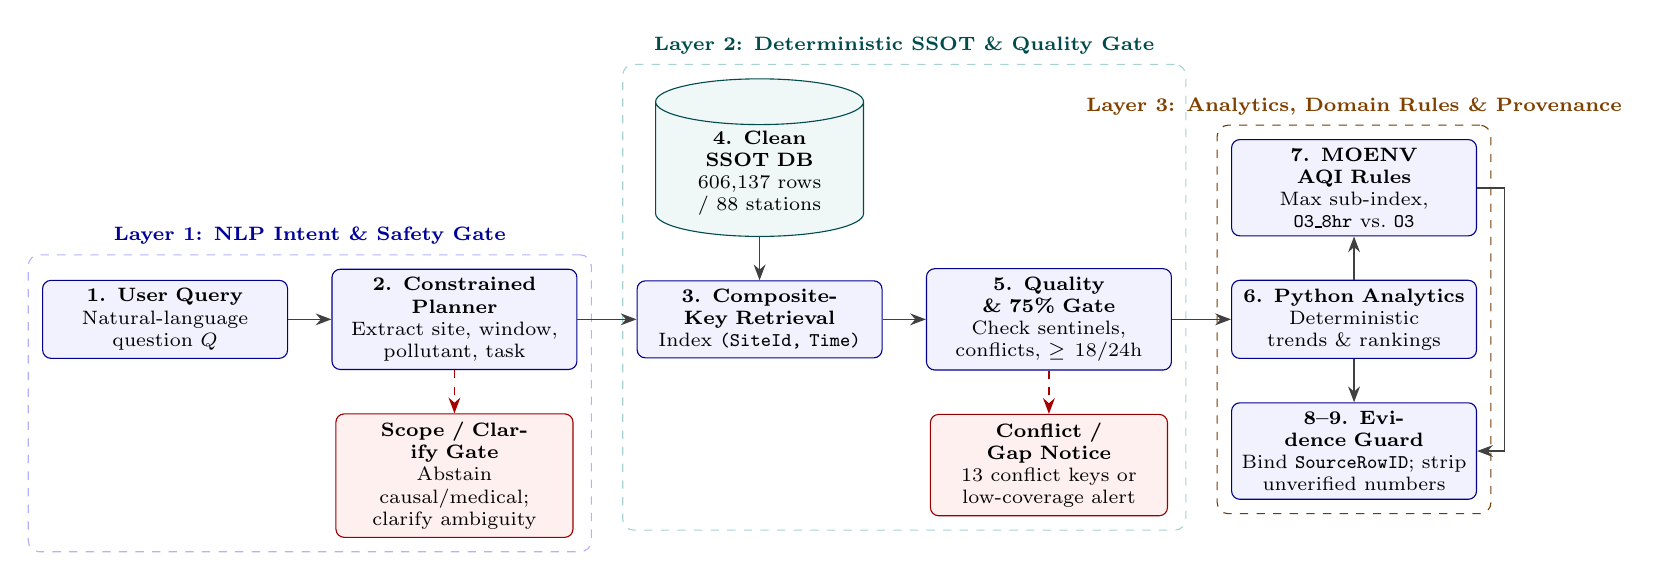
\begin{tikzpicture}[
    node distance=0.45cm and 0.55cm,
    box/.style={rectangle, rounded corners=3pt, draw=blue!55!black, fill=blue!5, text width=2.9cm, align=center, font=\scriptsize, minimum height=0.88cm, inner sep=3pt},
    store/.style={cylinder, shape border rotate=90, aspect=0.22, draw=teal!60!black, fill=teal!6, text width=2.5cm, align=center, font=\scriptsize, minimum height=0.85cm, inner sep=2pt},
    guard/.style={rectangle, rounded corners=3pt, draw=red!60!black, fill=red!6, text width=2.8cm, align=center, font=\scriptsize, minimum height=0.82cm, inner sep=3pt},
    arrow/.style={-{Stealth[length=2mm]}, semithick, draw=black!75},
    dashedarrow/.style={-{Stealth[length=2mm]}, semithick, dashed, draw=red!65!black}
]
% Layer 1
\node[box] (u) {\textbf{1. User Query}\\Natural-language question $Q$};
\node[box, right=of u] (p) {\textbf{2. Constrained Planner}\\Extract site, window, pollutant, task};
\node[guard, below=0.55cm of p] (sg) {\textbf{Scope / Clarify Gate}\\Abstain causal/medical; clarify ambiguity};

% Layer 2
\node[box, right=0.75cm of p] (r) {\textbf{3. Composite-Key Retrieval}\\Index \texttt{(SiteId, Time)}};
\node[store, above=0.55cm of r] (db) {\textbf{4. Clean SSOT DB}\\606,137 rows / 88 stations};
\node[box, right=of r] (q) {\textbf{5. Quality \& 75\% Gate}\\Check sentinels, conflicts, $\ge 18/24$h};
\node[guard, below=0.55cm of q] (cf) {\textbf{Conflict / Gap Notice}\\13 conflict keys or low-coverage alert};

% Layer 3
\node[box, right=0.75cm of q] (a) {\textbf{6. Python Analytics}\\Deterministic trends \& rankings};
\node[box, above=0.55cm of a] (k) {\textbf{7. MOENV AQI Rules}\\Max sub-index, \texttt{O3\_8hr} vs.\ \texttt{O3}};
\node[box, below=0.55cm of a] (g) {\textbf{8--9. Evidence Guard}\\Bind \texttt{SourceRowID}; strip unverified numbers};

\draw[arrow] (u) -- (p);
\draw[dashedarrow] (p) -- (sg);
\draw[arrow] (p) -- (r);
\draw[arrow] (db) -- (r);
\draw[arrow] (r) -- (q);
\draw[dashedarrow] (q) -- (cf);
\draw[arrow] (q) -- (a);
\draw[arrow] (a) -- (k);
\draw[arrow] (k.east) -- ++(0.35,0) |- (g.east);
\draw[arrow] (a) -- (g);

\begin{scope}[on background layer]
    \node[draw=blue!30, dashed, rounded corners=4pt, fit=(u)(p)(sg), inner sep=5pt, label={[font=\scriptsize\bfseries, text=blue!60!black]above:Layer 1: NLP Intent \& Safety Gate}] {};
    \node[draw=teal!35, dashed, rounded corners=4pt, fit=(r)(db)(q)(cf), inner sep=5pt, label={[font=\scriptsize\bfseries, text=teal!60!black]above:Layer 2: Deterministic SSOT \& Quality Gate}] {};
    \node[draw=orange!45!black, dashed, rounded corners=4pt, fit=(a)(k)(g), inner sep=5pt, label={[font=\scriptsize\bfseries, text=orange!50!black]above:Layer 3: Analytics, Domain Rules \& Provenance}] {};
\end{scope}
\end{tikzpicture}
\caption{Nine-stage decoupled architecture of AirGuard AI separating LLM query planning from deterministic data retrieval, statutory MOENV AQI rules, and row-level provenance verification.}
\label{fig:architecture}
\end{figure*}

\subsection{Mathematical Formulation and Statutory Rules}
Following Taiwan MOENV AQI breakpoint standards~\cite{moenv_aqi_def}, each pollutant sub-index $I_p$ is computed via piecewise linear interpolation:
\begin{equation}
I_p = \frac{I_{\text{high}} - I_{\text{low}}}{C_{\text{high}} - C_{\text{low}}} \left(C_p - C_{\text{low}}\right) + I_{\text{low}},
\label{eq:subindex}
\end{equation}
where $C_p$ is the pollutant concentration over its statutory averaging window (strictly separating hourly \texttt{O3} from 8-hour moving-average \texttt{O3\_8hr}, \texttt{CO\_8hr}, and \texttt{PM2.5\_AVG}), and $[C_{\text{low}}, C_{\text{high}}]$, $[I_{\text{low}}, I_{\text{high}}]$ denote the corresponding concentration and index breakpoints. The station AQI and governing pollutant $P_{\text{governing}}$ obey the maximum-sub-index rule:
\begin{equation}
\text{AQI} = \max_{p \in \mathcal{P}} I_p, \qquad
P_{\text{governing}} = \arg\max_{p \in \mathcal{P}} I_p,
\label{eq:aqi}
\end{equation}
for $\mathcal{P} = \{\text{PM}_{2.5}, \text{PM}_{10}, \text{O}_3, \text{CO}, \text{SO}_2, \text{NO}_2\}$.

To prevent biased daily summaries under sensor maintenance or power outages, daily statistics require at least 75\% hourly validity:
\begin{equation}
\text{CoverageRate}(s, d) = \frac{N_{\text{valid\_hours}}(s, d)}{24} \ge 0.75 \quad (\ge 18\text{ hours}).
\label{eq:coverage}
\end{equation}
Finally, provenance faithfulness over $N$ numeric claims generated in a response is defined as:
\begin{equation}
\text{Faithfulness} = \frac{\sum_{i=1}^{N} \mathbb{I}(\text{Claim}_i \text{ matches } \text{RetrievedRow}_i)}{\sum_{i=1}^{N} \mathbb{I}(\text{Claim}_i \text{ is numeric})}.
\label{eq:faithfulness}
\end{equation}

\subsection{Deterministic Execution Algorithm}
Algorithm~\ref{alg:airguard} formalizes the end-to-end inference loop, ensuring that no LLM-synthesized number reaches the user without matching a verified \texttt{SourceRowID}.

\begin{algorithm}[!t]
\caption{AirGuard AI Deterministic Provenance-Grounded Execution}
\label{alg:airguard}
\begin{algorithmic}[1]
\Require User query $Q$, clean dataset $D_{\text{clean}}$ (606,137 rows), conflict log $D_{\text{conflict}}$ (13 keys)
\Ensure Provenance-verified response $R$
\State $\text{plan} \gets \text{Planner.Parse}(Q)$ \Comment{\{site\_id, window, pollutant, task\}}
\If{$\text{plan.is\_medical}$ \textbf{or} $\text{plan.is\_causal\_blame}$}
    \State \Return $\text{ScopeGuard.Abstain}(\text{plan.boundary\_type})$
\EndIf
\If{\textbf{not} $\text{IsValidSite}(\text{plan.site\_id})$ \textbf{or not} $\text{IsValidWindow}(\text{plan.window})$}
    \State \Return $\text{Planner.ClarifyOrDiscloseDefault}(\text{plan})$
\EndIf
\State $\text{conflicts} \gets D_{\text{conflict}}.\text{Lookup}(\text{plan.site\_id}, \text{plan.window})$
\If{$\text{conflicts} \neq \emptyset$}
    \State \Return $\text{QualityFilter.ConflictNotice}(\text{conflicts})$
\EndIf
\State $\text{records} \gets D_{\text{clean}}.\text{Retrieve}(\text{plan.site\_id}, \text{plan.window})$
\If{$\text{records} = \emptyset$ \textbf{or} $\text{CoverageRate}(\text{records}) < 0.75$}
    \State \Return $\text{QualityFilter.DataGapNotice}(\text{records})$
\EndIf
\State $\text{stats} \gets \text{PythonAnalytics.Compute}(\text{records}, \text{plan})$
\State $\text{aqi\_eval} \gets \text{MOENVRules.MaxSubIndex}(\text{records})$
\State $E \gets \emptyset$
\For{\textbf{each} $m \in \text{stats.metrics}()$}
    \State $\text{row} \gets \text{records.FindSupportingRow}(m.\text{site}, m.\text{time}, m.\text{field})$
    \State $E \gets E \cup \{(m.\text{value}, m.\text{unit}, m.\text{site}, m.\text{time}, \text{row.id})\}$
\EndFor
\State $\text{draft} \gets \text{Synthesizer.Generate}(\text{stats}, \text{aqi\_eval}, E)$
\State $R \gets \text{EvidenceGuard.VerifyAndStrip}(\text{draft}, E)$
\State \Return $R$
\end{algorithmic}
\end{algorithm}

\subsection{OpenSpec Spec-Driven Development Workflow}
To keep engineering design, regulatory constraints, and manuscript claims synchronized, AirGuard AI adopts OpenSpec SDD (\texttt{openspec/specs/}) as its single source of specification truth. Five canonical specifications---covering \texttt{data-pipeline}, \texttt{agent-architecture}, \texttt{domain-rules}, \texttt{evaluation-benchmark}, and \texttt{ieee-conference-draft}---codify verifiable \textsc{When/Then} scenarios validated via \texttt{openspec validate --all --strict}. Changes from engineering design (\texttt{DESIGN.md}) to this IEEE conference draft are tracked through versioned OpenSpec change proposals on GitHub, guaranteeing full traceability between system requirements and manuscript specifications.

\section{Evaluation Plan and Expected Outcomes}
\subsection{\texttt{AirGuard-Eval-60} Benchmark Protocol}
We design a fixed, reproducible 60-question benchmark (\texttt{AirGuard-Eval-60}) grounded in deterministic reference queries over the January--October 2026 \texttt{AQX\_P\_488} snapshot, manually audited for station codes, time boundaries, and statutory rules:
\begin{itemize}
    \item \textbf{Answerable Queries (45 questions):} Temporal trend analysis (15 questions covering daily/weekly deltas and peak hours), cross-station spatial comparisons (15 questions covering intra-county rankings and concentration gaps), and MOENV AQI/dominant-pollutant interpretation (15 questions distinguishing \texttt{O3\_8hr} from hourly \texttt{O3} and \texttt{PM2.5\_AVG}).
    \item \textbf{Boundary and Abstention Cases (15 questions):} Sensor outages below the 75\% coverage gate (5 questions), queries intersecting the 13 quarantined conflict keys (3 questions), leading factory causal-attribution prompts (4 questions), and clinical diagnosis or medication inquiries (3 questions).
\end{itemize}

\subsection{Baselines and Metrics}
Three experimental conditions will be evaluated under identical prompt inputs:
\begin{enumerate}
    \item \textbf{Baseline 1 (LLM-Only):} Frontier LLM queried directly without historical CSV retrieval or deterministic tools.
    \item \textbf{Baseline 2 (Deterministic Tools Only):} Python/Pandas reference scripts returning structured JSON/tables without natural-language narrative.
    \item \textbf{Proposed (AirGuard AI):} Full decoupled pipeline integrating the constrained Planner, SSOT retrieval, MOENV rules, and Evidence/Scope Guards.
\end{enumerate}

Four metrics govern evaluation: (1) \emph{Numeric Accuracy} (concentration within $\pm 0.1\,\mu\text{g/m}^3$, exact integer AQI match), (2) \emph{Provenance Linkage Accuracy} (exact match of cited \texttt{SiteId}, timestamp, and \texttt{SourceRowID}), (3) \emph{Unsupported Claim Rate} (numeric tokens lacking a supporting retrieved row), and (4) \emph{Abstention Precision} across the 15 boundary cases.

\begin{table*}[!t]
\centering
\caption{Planned Evaluation Targets and Qualitative Expectations on \texttt{AirGuard-Eval-60} (Proposal Stage Only---No Executed Results)}
\label{tab:eval_targets}
\footnotesize
\renewcommand{\arraystretch}{1.15}
\begin{tabularx}{\textwidth}{@{}L{3.2cm} Y Y Y@{}}
\toprule
\textbf{Evaluation Dimension} & \textbf{Baseline 1: LLM-Only (Expected Behavior)} & \textbf{Baseline 2: Tools Only (Expected Behavior)} & \textbf{Proposed: AirGuard AI (Planned Acceptance Target)} \\
\midrule
Numeric Accuracy & Low (no historical access; arithmetic drift) & 100\% (direct query execution) & Target $>90\%$ (deterministic parity) \\
Provenance Linkage Accuracy & Very low (no row-ID binding) & 100\% (raw tabular fields) & Target $100\%$ (mandatory \texttt{SourceRowID}) \\
Unsupported Claim Rate & Significant hallucination risk & $0.0\%$ (no prose synthesis) & Target $0.0\%$ (Evidence Guard stripping) \\
Boundary Abstention Precision & Low (prone to forced guessing) & Moderate (raw empty/error codes) & Target $>90\%$ (transparent conflict/scope alerts) \\
Natural-Language Readability & High (fluent prose, ungrounded) & Poor (raw JSON/CSV output) & High (fluent prose + auditable provenance) \\
\bottomrule
\end{tabularx}
\end{table*}

Table~\ref{tab:eval_targets} summarizes the planned acceptance criteria. Consistent with strict academic integrity, these values represent design targets to be tested after implementation rather than measured results.

\section{Limitations, Future Work, and Conclusion}
\subsection{Current Limitations and Future Extensions}
First, the audited \texttt{AQX\_P\_488} snapshot (January 1 to October 29, 2026) represents a partial year and cannot support full-year seasonal generalizations. Second, the timestamp field \texttt{DataCreationDate} is preserved verbatim; confirming whether MOENV defines it strictly as physical sampling end-time or publication time is required before renaming schema semantics. Third, live streaming integration via \texttt{AQX\_P\_432} and Tier-2 fusion with calibrated AirBox micro-sensors~\cite{tzeng2023airbox,dong2025calibration,fang2025deployment,lekamge2025rh} remain future extensions contingent on verified API rate limits and collocated drift models.

\subsection{Conclusion}
We presented \textbf{AirGuard AI}, an OpenSpec-governed, deterministic, and row-level provenance-grounded conversational agent tailored to Taiwan's MOENV \texttt{AQX\_P\_488} hourly air-quality records and 2025 tightened standards. By decoupling constrained LLM query planning from audited Python analytics, quarantining 13 native conflict keys across 970,296 raw rows, enforcing a 75\% daily completeness gate, and binding every numeric claim to its \texttt{(SiteId, DataCreationDate, SourceRowID)}, AirGuard AI establishes a rigorous, auditable blueprint for trustworthy environmental question answering.

\bibliographystyle{IEEEtran}
\bibliography{references}

\end{document}
